\section{Skalenfreie Graphen und Feldexperiment}
\authors{Charlotte Häußler und Philipp Davydov}
\subsection{Einführung und Idee}
Bereits lange vor Beginn der Akademie Grovesmühle wurden die TN über das bevorstehende Feldexperiment des Kurses 3.1 informiert. Es handelt sich um ein akademieweites Projekt zur Untersuchung sozialer Graphen, im Zuge dessen alle Freiwilligen mit Bluetooth-Beacons ausgestattet wurden. Diese Beacons kommunizieren auf einer Distanz von bis zu zwei Metern. Dabei werden jedesmal Zeitpunkt und Dauer der Verbindung zweier Beacons registriert. Die so anonym erhobenen Daten wurden von den KL aufbereitet, erneut anonymisiert und schließlich an die TN des Kurses zur Auswerung übergeben.
\subsection{Skalenfreie Graphen}
Das Ziel des Feldexperiments war die Untersuchung sozialer Graphen, also Graphen, die soziale Netzwerke darstellen, auf Skalenfreiheit. Da es sich bei dieser Form von Graphen um ein recht neues Gebiet der Mathematik handelt, gibt es noch keine vollständig einheitliche Definition. Zur Betrachtung der Ergebnisse wird die allgemein gängiste Definition verwendet.
\begin{df} Sei $G=(V,E)$ ein zusammenhängender Graph und $P(k)$ der Anteil der Knoten mit Grad k. Dann heißt $G$ skalenfrei, falls die Knotengrade einem Potenzgesetz folgen, das folgendermaßen beschrieben werden kann
\begin{align*}
P(k) \varpropto k^{-\alpha}
\end{align*}
mit Skalierungsfaktor $\alpha$. Dabei gilt normalerweise $1\leq\alpha\leq3$.
\end{df}
Anders ausgedrückt verhält sich die Zahl der Knoten mit einem bestimmten Grad in $G$ ähnlich wie die Funktion $f(x) = \frac{1}{x^{|\alpha|}}$ .
\subsection{Soziale Graphen}
Skalenfreie Graphen entstehen durch den Zufallsprozess des \textit{preferencial attachment}. Dabei existieren zu Beginn einige initiale Knoten. Danach werden iterativ Knoten ergänzt, die zufällig Kanten bilden. Neu hinzukommende Knoten verknüpfen sich hierbei bevorzugt mit Knoten die bereits einen hohen Grad haben. Je mehr Nachbarn ein Knoten also bereits hat, desto wahrscheinlicher ist das Hinzukommen weiter Nachbarknoten. Somit können auch soziale Graphen als skalenfrei angesehen werden. Neue Menschen, die einer sozialen Gruppe beitreten, wahrscheinlich zuerst mit denjenigen Kontakte knüpfen werden, die momentan die meisten Kontakte haben bzw. beliebt sind. Die Beliebten werden dann von den Knoten mit hohem Grad repsäsentiert.
\subsection{Vergleich mit Fraktalen}
Fraktale sind selbstähnliche Strukturen, das heißt, dass ihre Struktur in größeren Maßstäben ähnlich der des Anfangzustandes ist. Ein gutes Beispiel ist die Kochkurve in Abb. \ref{KK}.

Eine  Ansicht, die durch die Analogie zwischen der Skalenfreiheit des Graphen und der Maßstabsfreiheit von Fraktalen motiviert ist ist, dass auch skalenfreie Graphen selbstähnlich sind.
Dabei ergibt sich allerdings das Problem, dass aus dem Potenzgesetz nicht unmittelbar die Selbstähnlichkeit folgt.
\begin{figure}
\centering
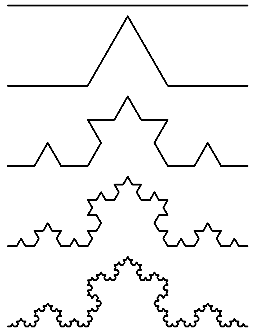
\includegraphics[scale=0.5]{img/Kochkurve}
\caption{Die selbstähnliche Struktur der Kochkurve (Quelle: \url{https://upload.wikimedia.org/wikipedia/commons/0/0f/Von\_Koch-kurvans\_utveckling.png})}
 \label{KK}
\end{figure}
\subsection {Das Feldexperiment}
Am Mittwoch den 11.07.2018 wurden die Beacons an die TN des Experiments verteilt und in die Namensschilder integriert. So wurde erreicht, dass die TN ihre Beacons etwa 17 Stunden pro Tag bei sich trugen, wodurch sehr gute Ergebnisse entstanden. Etwa eine Woche später wurde das Experiment beendet, die Beacons eingesammelt und die Rohdaten von den KL in eine leichter zu verarbeitende Form gebracht. Am Ende dieses Prozesses stand eine Liste mit etwa 66000 Zeilen. Diese begannen mit einem Buchstaben zur Kategorisierung in die zwei Bestandteile (sozialer Graph und Seuchensimulation) des Experiments. In den Zeilen für den sozialen Graphen folgten dann die Nummern der beiden kommunizierenden Beacons, der Zeitpunkt der Kontaktaufnahme in Unixzeit (Verstrichene Zeit in Sekunden seit 00:00 Uhr des 1. Januar 1970) und die Dauer der Kopplung in Sekunden. Ein Beispiel wäre die folgende (fiktive) Zeile.
\begin{center}
N,9,124,1531654335,1783
\end{center}
Sie beinhaltet die Information, dass während des Experiments die Chips der (anonymisierten) Kennnummern 9 und 124 am 15.07.2018 ab etwa 13:32 Uhr (Unixzeit 1531654335) für eine knappe halbe Stunde (1783 Sekunden)  miteinander gekoppelt, also weniger als zwei Meter voneinander entfernt waren.
\begin{figure}
FEHLÈNDES BILD
\caption{Auswertung des Experiments, Graph zur Kurszeit}
\label{Auswertung}
\end{figure}

Zur Auswertung  wurde ein Python-Programm entwickelt, das aus den vorhandenen Daten verschiedene Graphen erstellt. Einer von ihnen ist  in Abb. \ref{Auswertung} dargestellt. Die Beacons werden durch Knoten und die Kopplungen durch Kanten repräsentiert. Es handelt sich um eine Momentaufnahme der bestehenden Verbindungen während der Kurszeit. Verknüpfte Knoten befanden sich demnach zu dieser Zeit in Kopplungsreichweite, also im selben Raum und somit im selben Kurs. Die Zusammenhangskomponenten stellen also die verschiedenen Kurse dar.
